% !TeX root = ../main.tex
% -*- coding: utf-8 -*-

\chapter{腔磁振子系统的稳态谱}
\label{ch4}

\section{关联函数的稳态解}
在\ref{ch3}\ref{sec3.2}中我们得到了腔磁振子系统的Fokker-Planck方程,这一节我们会从Fokker-Planck方程中导出包含系统任意阶关联函数的级联方程,并进一步求解系统稳态的二阶关联函数。

\subsection{级联方程}
Fokker-Planck方程\eqref{Fokker-Planck}的等号两边是关于$P$函数的微分,借助定义\eqref{MeanDefination}在Fokker-Planck方程两边同时积分计算变量$\alpha^{*p}\alpha^{q}\beta^{*r}\beta^{s}$的平均值就可以消去$P$,此时原本的独立变量$(\alpha,\alpha^{*},\beta,\beta^{*},t)$变得不再独立,以时间$t$为自变量我们可以得到如下的级联方程
\begin{equation}
\begin{aligned}
\dot{\overline{\alpha^{*p}\alpha^q\beta^{*r}\beta^s}}={}&\left[ (p-q)i\omega_{c}+(r-s)i\omega_{m}-(p+q)\kappa_{c}-(r+s)\kappa_{m}\right]\overline{\alpha^{*p}\alpha^q\beta^{*r}\beta^s} \\ &+pig\overline{\alpha^{*p-1}\alpha^q\beta^{*r+1}\beta^s} -qig\overline{\alpha^{*p}\alpha^{q-1}\beta^{*r}\beta^{s+1}} \\ &+rig\overline{\alpha^{*p+1}\alpha^q\beta^{*r-1}\beta^s} -sig\overline{\alpha^{*p}\alpha^{q+1}\beta^{*r}\beta^{s-1}}  \\
&+p\Omega e^{i\omega_{0}t}\overline{\alpha^{*p-1}\alpha^q\beta^{*r}\beta^s} +q\Omega e^{-i\omega_{0}t}\overline{\alpha^{*p}\alpha^{q-1}\beta^{*r}\beta^s} \\
&+2pq\kappa_{c}\overline{n}_{c}\overline{\alpha^{*p-1}\alpha^{q-1}\beta^{*r}\beta^s}
+2rs\kappa_{m}\overline{n}_{m}\overline{\alpha^{*p}\alpha^q\beta^{*r-1}\beta^{s-1}}
\label{HierarchicalEq}
\end{aligned}
\end{equation}
上面的级联方程中$(p+q+r+s)$阶的变量只与同阶量以及低阶量有关,所以$(p+q+r+s)$阶的变量只需要有限多个方程联立即可求解。而对于我们关注的系统在长时间演化后所到达的稳态,可以假设有如下形式解:
\begin{equation}
\alpha(t)=\alpha_{0}e^{-i\omega_{0}t}, \quad \beta(t)=\beta_{0}e^{-i\omega_{0}t}
\label{SolutionForm}
\end{equation}
在这里我们认为稳态时系统的振荡行为和外加驱动同步,$\alpha_{0}$和$\beta_{0}$是与时间无关的变量。

将形式解\eqref{SolutionForm}代入级联方程\eqref{HierarchicalEq}中,就可以得到稳态的级联方程。其中一阶变量所满足的方程组为
\begin{equation}
\begin{aligned}
-i\omega_{0}\overline{\alpha_{0}}&=-i\omega_{c}\overline{\alpha_{0}}-ig\overline{\beta_{0}}+\Omega-\kappa_{c}\overline{\alpha_{0}} \\
i\omega_{0}\overline{\alpha^{*}_{0}}&=i\omega_{c}\overline{\alpha^{*}_{0}}+ig\overline{\beta^{*}_{0}}+\Omega-\kappa_{c}\overline{\alpha^{*}_{0}} \\
-i\omega_{0}\overline{\beta_{0}}&=-i\omega_{m}\overline{\beta_{0}}-ig\overline{\alpha_{0}}-\kappa_{m}\overline{\beta_{0}} \\
i\omega_{0}\overline{\beta^{*}_{0}}&=i\omega_{m}\overline{\beta^{*}_{0}}+ig\overline{\alpha^{*}_{0}}-\kappa_{m}\overline{\beta^{*}_{0}} \label{1odeqs}
\end{aligned}
\end{equation}
联立求解可得到
\begin{equation}
\begin{aligned}
\overline{\alpha_{0}} = \frac{\Omega(\kappa_{m}+i(\omega_{m}-\omega_{0}))}{(\kappa_{c}+i(\omega_{c}-\omega_{0}))(\kappa_{m}+i(\omega_{m}-\omega_{0}))+g^{2}} \\
\overline{\alpha^{*}_{0}} = \frac{\Omega(\kappa_{m}-i(\omega_{m}-\omega_{0}))}{(\kappa_{c}-i(\omega_{c}-\omega_{0}))(\kappa_{m}-i(\omega_{m}-\omega_{0}))+g^{2}} \\
\overline{\beta_{0}} = \frac{-ig\Omega}{(\kappa_{c}+i(\omega_{c}-\omega_{0}))(\kappa_{m}+i(\omega_{m}-\omega_{0}))+g^{2}} \\ 
\overline{\beta^{*}_{0}} = \frac{ig\Omega}{(\kappa_{c}-i(\omega_{c}-\omega_{0}))(\kappa_{m}-i(\omega_{m}-\omega_{0}))+g^{2}} 
\end{aligned}\label{first_order}
\end{equation}
同样地,二阶变量在稳态时所满足的级联方程组为
\begin{equation}
\begin{aligned}
{\overline{\alpha^{*}_0\alpha_0}}={}&-ig\overline{\alpha^{*}_0\beta_0}+ig\overline{\alpha_0\beta_0^{*}}+\Omega \overline{\alpha^{*}_0}+\Omega \overline{\alpha_0}-2\kappa_{c}\overline{\alpha^{*}_0\alpha_0}
+2\kappa_{c}\overline{n}_{c} \\
{\overline{\beta_0^{*}\beta_0}}={}&ig\overline{\alpha^{*}_0\beta_0} -ig\overline{\alpha_0\beta_0^{*}} -2\kappa_{m}\overline{\beta_0^{*}\beta_0}
+2\kappa_{m}\overline{n}_{m} \\
{\overline{\alpha^{*}_0\beta_0}}={}&i\omega_{c}\overline{\alpha^{*}_0\beta_0} -i\omega_{m}\overline{\alpha^{*}_0\beta_0} -ig\overline{\alpha^{*}_0\alpha_0}+ig\overline{\beta_0^{*}\beta_0}+\Omega \overline{\beta_0}-\kappa_{c}\overline{\alpha^{*}_0\beta_0}-\kappa_{m}\overline{\alpha^{*}_0\beta_0} \\
{\overline{\alpha_0\beta_0^{*}}}={}&-i\omega_{c}\overline{\alpha_0\beta_0^{*}}+i\omega_{m}\overline{\alpha_0\beta_0^{*}}
+ig\overline{\alpha^{*}_0\alpha_0}-ig\overline{\beta_0^{*}\beta_0}+\Omega \overline{\beta_0^{*}}-\kappa_{c}\overline{\alpha_0\beta_0^{*}}-\kappa_{m}\overline{\alpha_0\beta_0^{*}}
\end{aligned}\label{2odeqs}
\end{equation}
结合一阶变量的解\eqref{first_order}即可求得上面方程组的解为
\begin{align}
\langle c^{\dag}c \rangle = \overline{\alpha_{0}^{*}\alpha_{0}}&=|\overline{\alpha_{0}}|^{2}+(1-\gamma_{m})\overline{n}_c+\gamma_{m}\overline{n}_m \label{photon_num} \\
\langle m^{\dag}m \rangle = \overline{\beta_{0}^{*}\beta_{0}}&=|\overline{\beta_{0}}|^{2}+(1-\gamma_{c})\overline{n}_m+\gamma_{c}\overline{n}_c \label{magnon_num}
\end{align}
其中的参数为
\begin{align}
\gamma_m&=\frac{g^2\kappa_m(\kappa_c+\kappa_m)}{g^2(\kappa_c+\kappa_m)^2+\kappa_c\kappa_m(\kappa_c+\kappa_m)^2+\kappa_c\kappa_m(\omega_{m}-\omega_{c})^2} \\
\gamma_c&=\frac{g^2\kappa_c(\kappa_c+\kappa_m)}{g^2(\kappa_c+\kappa_m)^2+\kappa_c\kappa_m(\kappa_c+\kappa_m)^2+\kappa_c\kappa_m(\omega_{m}-\omega_{c})^2}
\end{align}

这里简单说明一下,对于腔磁振子理论中通常使用的量子朗之万方程方法,经常会对海森堡绘景下的算符演化方程做傅立叶变换\cite{10.1126/sciadv.1501286Tang,Zhang2019Theory},此时如果取算符平均值就能得到与方程组\eqref{1odeqs}类似的一阶量方程组,但是如果想要同样使用量子朗之万方程来得到与方程组\eqref{2odeqs}类似的二阶量方程组的话,原则上就需要处理算符形式的随机微积分,而这种做法目前在数学和物理的相关文献中均未见有人使用过。

\subsection{二阶关联函数}
目前实验上对腔磁振子系统的测量主要集中在微波腔的透射谱和反射谱上,这些测得的微波强度量正比于腔中的光子数\cite{harder2016study}。而HBT实验告诉我们一阶关联(相干)$\langle c^{\dag}c \rangle$并不能反映出光场的量子特性,我们必须要使用更高阶的关联函数才能对量子系统做出更全面的描述。在量子光学理论中,定义了光场的二阶关联函数为\cite{gerry2005introductory}
\begin{equation}
g^{(2)}_{pho}(\tau)=\frac{\left\langle\hat{E}^{(-)}(t) \hat{E}^{(-)}(t+\tau) \hat{E}^{(+)}(t+\tau) \hat{E}^{(+)}(t)\right\rangle}{\left\langle\hat{E}^{(-)}(t) \hat{E}^{(+)}(t)\right\rangle\left\langle\hat{E}^{(-)}(t+\tau) \hat{E}^{(+)}(t+\tau)\right\rangle}
\end{equation}
它表征着在同一位置的两个不同时刻都检测到光子的概率。而使用类似的形式我们也可以定义磁化强度场算符的二阶关联函数
\begin{equation}
g^{(2)}_{mag}(\tau)=\frac{\left\langle\hat{M}^{(-)}(t) \hat{M}^{(-)}(t+\tau) \hat{M}^{(+)}(t+\tau) \hat{M}^{(+)}(t)\right\rangle}{\left\langle\hat{M}^{(-)}(t) \hat{M}^{(+)}(t)\right\rangle\left\langle\hat{M}^{(-)}(t+\tau) \hat{M}^{(+)}(t+\tau)\right\rangle}
\end{equation}
当时延$\tau=0$时,单模场中光子和磁振子的二阶关联函数就可以写为
\begin{align}
g_{pho}^{(2)}(0) & = \frac{\langle c^{\dag2}c^2\rangle}{\langle c^{\dag}c\rangle^2} =\frac{\overline{\alpha_{0}^{*}\alpha_{0}^{*}\alpha_{0}\alpha_{0}}}{\overline{\alpha_{0}^{*}\alpha_{0}}^2} \\
g_{mag}^{(2)}(0) & =\frac{\langle m^{\dag2}m^2\rangle}{\langle m^{\dag}m\rangle^2} =\frac{\overline{\beta_{0}^{*}\beta_{0}^{*}\beta_{0}\beta_{0}}}{\overline{\beta_{0}^{*}\beta_{0}}^2}
\end{align}

可以看出要想计算二阶关联函数,我们必须得到稳态的四阶变量平均值,而重复上一小节的做法,在求解三阶变量以及四阶变量稳态的级联方程组后,我们就可以得到$\overline{\alpha_{0}^{*}\alpha_{0}^{*}\alpha_{0}\alpha_{0}}$与$\overline{\beta_{0}^{*}\beta_{0}^{*}\beta_{0}\beta_{0}}$。但是我们目前并不能把解化简为像一阶和二阶变量那样的简单形式,只能编写程序来数值计算。而为了方便我们的解析理解,可以限制参数范围$\omega_{c}=\omega_{m}$,也就是腔中光场和磁振子共振的时候,在这一特殊参数下可以得到稳态时简洁形式的二阶与四阶变量解为
\begin{align}
\overline{\alpha_{0}^{*}\alpha_{0}}&=|\overline{\alpha_{0}}|^{2}+n \\
\overline{\beta_{0}^{*}\beta_{0}}&=|\overline{\beta_{0}}|^{2}+n \\
\overline{\alpha_{0}^{*}\alpha_{0}^{*}\alpha_{0}\alpha_{0}}&=(|\overline{\alpha_{0}}|^{2}+2n)^2-2n^2 \\
\overline{\beta_{0}^{*}\beta_{0}^{*}\beta_{0}\beta_{0}}&=(|\overline{\beta_{0}}|^{2}+2n)^2-2n^2
\end{align}
由于此时光子和磁振子的热占据数相等,因此表示为$n=\overline{n}_{c}=\overline{n}_{m}$。同时,光子和磁振子的零时延二阶关联函数为
\begin{align}
g_{pho}^{(2)}(0) &  =\frac{(|\overline{\alpha_{0}}|^{2}+2n)^2-2n^2}{(|\overline{\alpha_{0}}|^{2}+n)^2} \label{g2pho} \\
g_{mag}^{(2)}(0) &  =\frac{(|\overline{\beta_{0}}|^{2}+2n)^2-2n^2}{(|\overline{\beta_{0}}|^{2}+n)^2} \label{g2mag}
\end{align}
而对于时延$\tau>0$的情况,只使用目前的级联方程我们尚未找到合适的方法来计算,但是有了零时延二阶关联函数$g^{(2)}(0)$以后,量子光学中通常会借助所谓的量子回归公式(Quantum Regression Formula)来得到特殊情况下时延$\tau>0$的结果\cite{carmichael1999statistical},本文暂不作讨论\ChangeNotation。

%%%%%%%%%%%%%%%%%%%%%%%%%%%%
%new length to control the figures size below
\newlength{\basefigurewidth}
\setlength{\basefigurewidth}{0.33\textwidth}
%%%%%%%%%%%%%%%%%%%%%%%%%%%%

\section{腔磁振子系统中的耦合与耗散}
有了级联方程以及其稳态解之后,我们就可以计算系统中平均粒子数和二阶关联函数在稳态时随其他物理量的变化了。类似于测量中用到的谱的概念,当其他物理量是实验中连续可调的参数(驱动频率、驱动强度、偏置磁场等)时,我们称此时的计算结果为稳态谱\ChangeNotation。腔磁振子系统实验中测量的稳态时的透射谱和反射谱,一般是在调节好外加偏置磁场后,使用矢量网络分析仪自动化测量微波腔中不同输入频率下的同频信号响应\cite{PhysRevB.99.134445Hu}。为了和实验对比,这一节我们也按照这个思路计算稳态谱,级联方程解的参数空间由$\{ \omega_c,\omega_m,\omega_0,\kappa_c,\kappa_m,g,\Omega,T \}$构成,在计算时具体的参数选取基于Tang课题组的实验\cite{PhysRevLett.113.156401Tang}。

\subsection{强耦合参数下的相干竞争}
我们先来计算强耦合下$\langle c^{\dag}c \rangle$,$\langle m^{\dag}m \rangle$也就是光子和磁振子场的平均粒子数(能量)稳态谱。选取的参数为:$\omega_c/2\pi=7.875$ GHz, $\kappa_c/2\pi=1.35$ MHz, $\kappa_m/2\pi=1.06$ MHz, $g/2\pi=10.8$ MHz, $\Omega/2\pi=2$ THz 以及 $T=300$ K,让剩余的两个参数$\omega_m$,$\omega_0$在 7.83--7.92 GHz间围绕$\omega_c/2\pi$变化,并且把$\omega_m/2\pi$换算为实验中所调节的磁场,此时$\langle c^{\dag}c \rangle$,$\langle m^{\dag}m \rangle$的稳态谱分别如图\ref{SC1stOrder}(a)和(b)所示。
\begin{figure}[htbp]
	\centering
	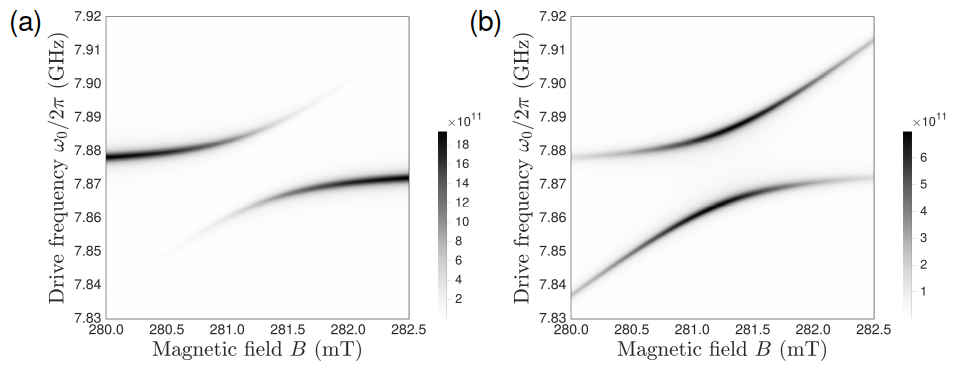
\includegraphics[width=2\basefigurewidth,clip]{./figure/4_1}
	\caption{强耦合参数下光子和磁振子平均粒子数的稳态谱} 
	\label{SC1stOrder}
\end{figure}
可以看到光子和磁振子平均粒子数的稳态谱中都出现了明显的反交错现象,并且光子的谱中围绕腔共振频率$\omega_c/2\pi$附近的强度最高,和实验上的特征一致,而磁振子谱则是围绕YIG球共振磁场附近的强度最高。

腔磁振子系统的稳态解\eqref{photon_num}以及\eqref{magnon_num}都可以看作是由两部分所构成,即相干部分$|\overline{\alpha_{0}}|^{2}$、$|\overline{\beta_{0}}|^{2}$以及由$\overline{n}_c$、$\overline{n}_m$决定的热部分。而在图\ref{SC1stOrder}的参数范围内可以计算出热占据数$\overline{n}_c\approx\overline{n}_m$在$793\pm5$小幅度变化,因此图\ref{SC1stOrder}的强度变化主要是由相干部分导致的。

对于稳态谱中的反交错现象可以这样理解,我们由孤立腔磁振子系统的哈密顿量
\begin{equation}
H_{iso} = \hbar\omega_{c}c^{\dag}c+\hbar\omega_{m}m^{\dag}m+\hbar gc^{\dag}m+\hbar gm^{\dag}c
\label{HamiltonianIsolated}
\end{equation}
可以将其变换为两个独立的polariton模式,并得到两个本征频率$\omega_p^{up}=\frac{1}{2}\Big[(\omega_c+\omega_m)+\sqrt{(\omega_c-\omega_m)^2+4g^2}\Big]$,$\omega_p^{down}=\frac{1}{2}\Big[(\omega_c+\omega_m)-\sqrt{(\omega_c-\omega_m)^2+4g^2}\Big]$。而在强耦合参数$g\gg\kappa_c,\kappa_m$下$\omega_p^{up}$,$\omega_p^{down}$正是\eqref{photon_num}与\eqref{magnon_num}关于驱动频率变量$\omega_0$的两个极大值点,因此不难理解当驱动频率调节到系统的本征频率附近时会出现共振并极大的增强系统中的光子和磁振子场。但是由于驱动场只输入相干光子,相干磁振子是通过耦合转化过来的,导致了图\ref{SC1stOrder}(a)和(b)中稳态谱强弱分布的差异。

有了能够和实验对比的光子和磁振子场的平均粒子数稳态谱后,我们接下来就有信心继续给出腔磁振子系统二阶关联函数的稳态谱。但是直接计算图\ref{SC1stOrder}所使用的实验参数下的二阶关联函数谱并不能得到很多信息,这点从\eqref{g2pho}和\eqref{g2mag}中就可以看出,因为此时的相干部分$|\overline{\alpha_{0}}|^{2},|\overline{\beta_{0}}|^{2} \gg n$,所以$g_{pho}^{(2)}(0)$和$g_{mag}^{(2)}(0)$在测量意义上等于1,也就是说此时的光子和磁振子都处于相干态。要想得到包含有用信息的二阶关联函数稳态谱,我们必须意识到目前的腔磁振子系统中存在着由外加驱动输入的相干部分以及由热环境导致的退相干部分的竞争,当某一部分过大时另一部分的要素就会被淹没在其中,这一点我们可以从图\ref{CoherentVary2edOrder}中看出。
\begin{figure}[htbp]
	\centering
	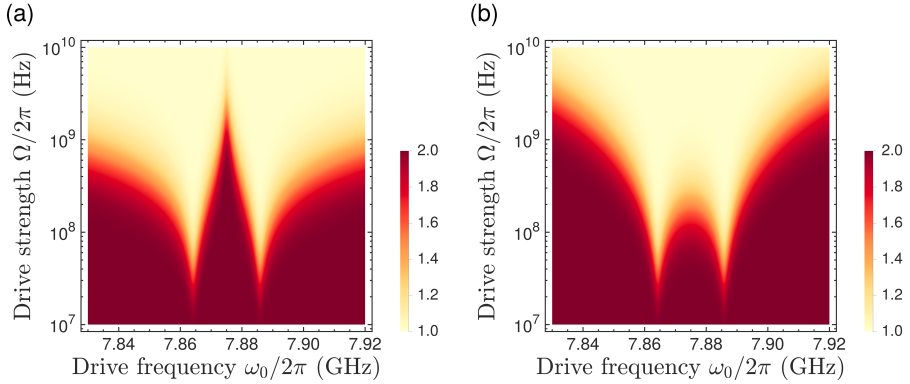
\includegraphics[width=2\basefigurewidth,clip]{./figure/4_2}
	\caption{光子和磁振子的二阶关联函数随驱动强度和驱动频率变化的二维颜色图} 
	\label{CoherentVary2edOrder}
\end{figure}
在图\ref{CoherentVary2edOrder}(a)和(b)中,我们分别绘制了当磁振子和腔中光子共振时二阶关联函数$g_{pho}^{(2)}(0)$和$g_{mag}^{(2)}(0)$在外加驱动强度$\Omega/2\pi$从$10^{10}$Hz减到$10^{7}$Hz的过程中随驱动频率$\omega_0/2\pi$变化的谱线,其他参数均和图\ref{SC1stOrder}一致。由于退相干部分保持不变,图\ref{CoherentVary2edOrder}实际上为我们展示了在相干部分“退潮”的过程中原本淹没在其中的退相干部分是如何逐渐显现出来的。当驱动强度过强时,$g_{pho}^{(2)}(0)=g_{mag}^{(2)}(0)=1$,系统中光子和磁振子都处于相干态,而当驱动强度过弱时,$g_{pho}^{(2)}(0)=g_{mag}^{(2)}(0)=2$,光子和磁振子又都处于热态。只有当相干部分和非相干部分竞争的不相上下时,二阶关联函数的稳态谱才会出现明显的强度分布。

\begin{figure}[htbp]
	\centering
	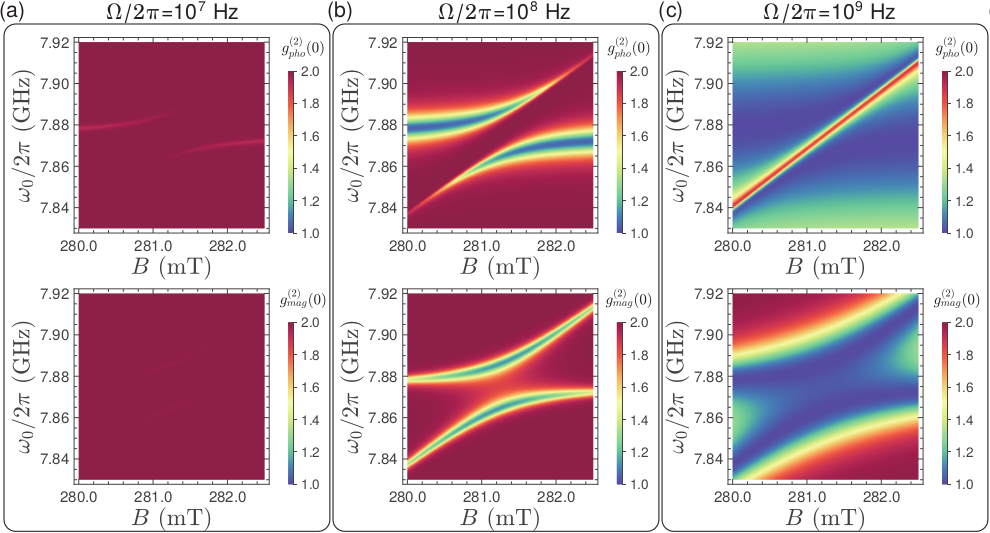
\includegraphics[width=3\basefigurewidth,clip]{./figure/4_3_1}
	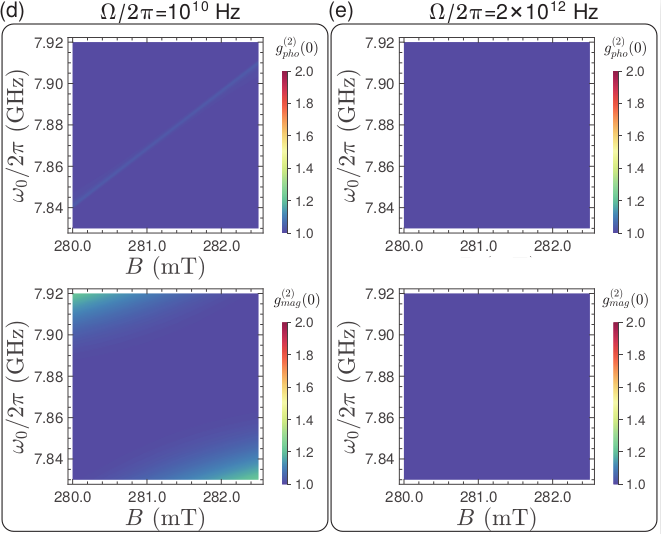
\includegraphics[width=2\basefigurewidth,clip]{./figure/4_3_2}
	\caption{不同驱动强度下的二阶关联函数稳态谱} 
	\label{Sepctrum2edOrder1}
\end{figure}
为了更直观和准确地理解腔磁振子系统中的相干竞争,我们可以像图\ref{SC1stOrder}一样计算二阶关联函数随外加驱动频率和偏置磁场变化的稳态谱。图\ref{Sepctrum2edOrder1}中我们展示了驱动强度$\Omega/2\pi$分别取$10^{7}$Hz,$10^{8}$Hz,$10^{9}$Hz,$10^{10}$Hz和$2$THz时具体的二阶关联函数稳态谱。其中当$\Omega/2\pi=10^{7}$Hz与$\Omega/2\pi=2$THz时,我们看到稳态谱都因为相干竞争的失衡而表现不出明显的变化。而在驱动强度增强的过程中,相干性增长最快的位置也处在polariton频率$\omega_p^{up}$和$\omega_p^{down}$上,图\ref{Sepctrum2edOrder1}(b)中二阶关联函数谱甚至表现出和平均粒子数谱一致的反交错现象。
\begin{figure}[htbp]
	\centering
	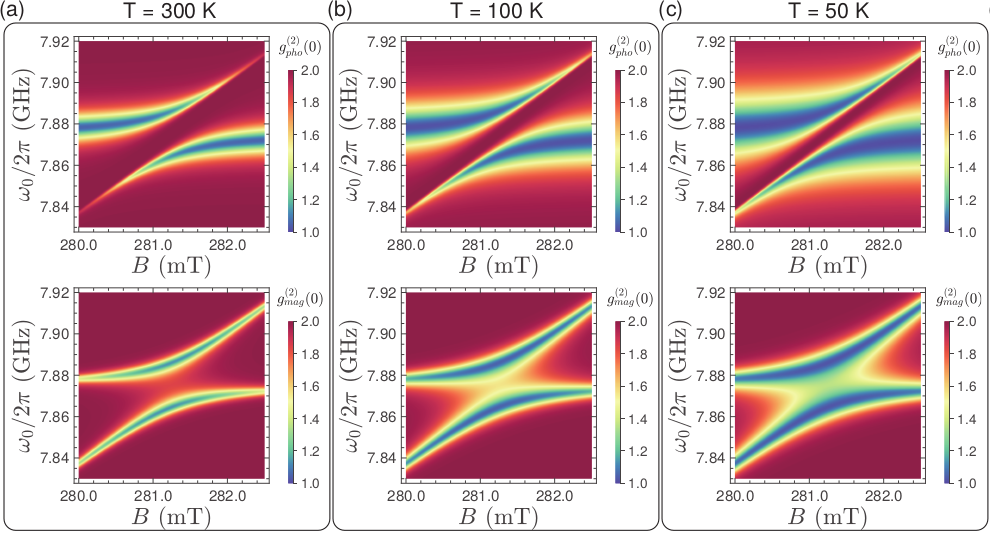
\includegraphics[width=3\basefigurewidth,clip]{./figure/4_4_1}
	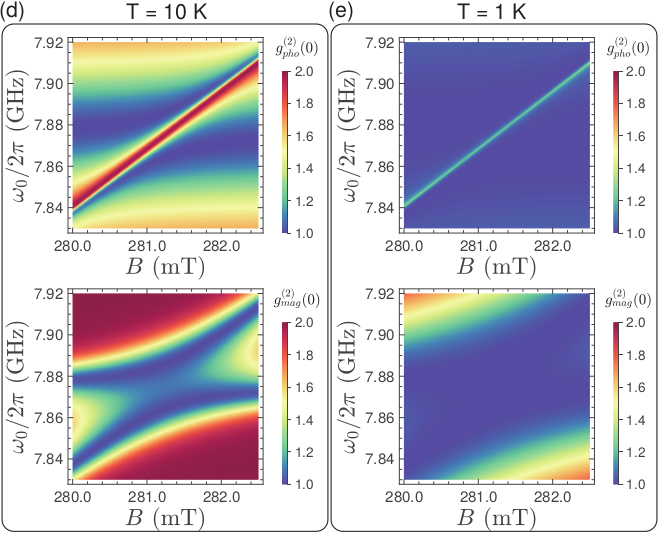
\includegraphics[width=2\basefigurewidth,clip]{./figure/4_4_2}
	\caption{不同温度下的二阶关联函数稳态谱} 
	\label{Sepctrum2edOrder2}
\end{figure}
在参数取定为图\ref{Sepctrum2edOrder1}(b)时,我们改变温度为$300$K,$100$K,$50$K,$10$K和$1$K,对应不同温度下的二阶关联函数稳态谱如图\ref{Sepctrum2edOrder2}(a)--(e)所示。可以看出,降低温度所引起的退相干部分减弱的效果与增强驱动的效果是一致的,当温度降低到退相干部分被完全压制的时候,腔磁振子系统就会表现为$g_{pho}^{(2)}(0)=g_{mag}^{(2)}(0)=1$的相干态。

\subsection{腔磁振子系统中的MIT现象}
由于腔磁振子系统的高度可调节性,Tang的实验中还实现了不同耦合参数下的测量。在耦合参数$\kappa_c>g>\kappa_m$时,系统中会出现MIT现象。MIT的称呼来源于以往的电磁诱导透明(EIT)现象,EIT指的是多能级原子和电磁场共振时,原本对探测电磁场的吸收会变为透明的现象,在实验中体现为测量谱线原本的洛伦兹线型会在峰值处出现一道尖锐的凹陷,腔磁振子系统中同样有着类似的实验现象。

我们选取参数为:$\omega_c/2\pi=\omega_m/2\pi=7.875$ GHz, $\kappa_m/2\pi=1.06$ MHz, $g/2\pi=10.8$ MHz, $\Omega/2\pi=1$ GHz 以及 $T=300$ K,绘制$\kappa_c/2\pi$增大的过程中光子和磁振子平均粒子数与二阶关联函数的稳态谱线如图\ref{MITkcVary}所示。
\begin{figure}[htbp]
	\centering
	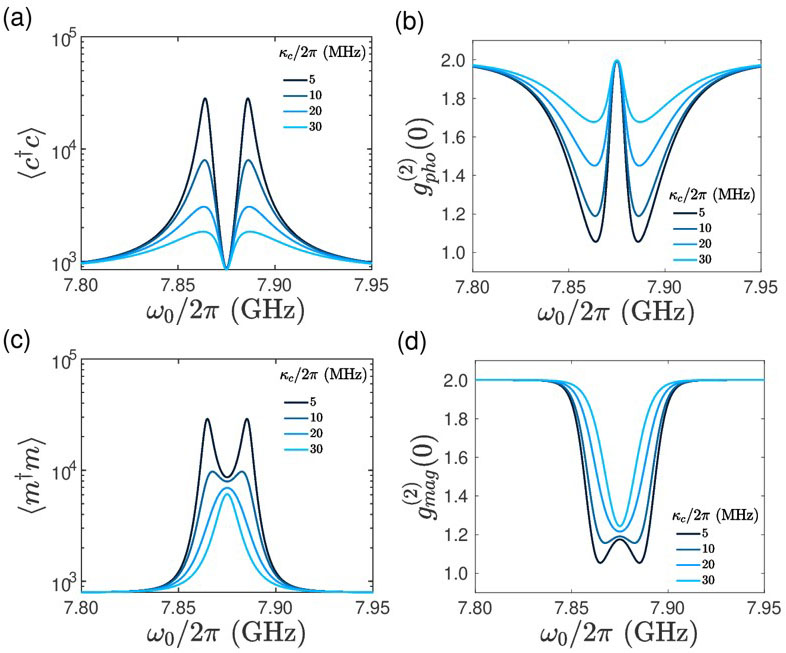
\includegraphics[width=2.1\basefigurewidth,clip]{./figure/4_5}
	\caption{微腔耗散率增大时光子和磁振子的稳态谱线} 
	\label{MITkcVary}
\end{figure}
可以看到,在单独增大微腔的耗散时,平均光子数一直保持着双峰的线型,但是两个对称峰的线宽一直在增大,峰值的位置依旧出现在$\omega_p^{up}$和$\omega_p^{down}$处。当$\kappa_c/2\pi=30$MHz时,耦合参数完全进入MIT区域,平均光子数的线型呈现极宽的线型中间出现一较窄线宽的凹陷,也就是经典EIT实验中的线型。在凹陷位置处$\omega_c=\omega_m=\omega_0$,由\eqref{first_order}可得光子相干部分$|\overline{\alpha_{0}}|^2 = \left(\frac{\Omega\kappa_{m}}{\kappa_{c}\kappa_{m}+g^{2}}\right)^2$保持十位数的量级,也就是说此处明明和其他位置处有着同样的耦合率、耗散率以及输入功率,与其他驱动频率处相比却几乎没有留住多少相干光子,造成这一结果的唯一原因在于稳态时的腔磁振子系统基本不再吸收输入光子,正是因为这样实验上此处的反射谱才会出现极大值,表示对输入光透明。尽管如此,我们只凭借平均光子数还是难以区分强耦合与MIT参数。但是在图\ref{MITkcVary}中我们发现平均磁振子数在两种参数下有着明显的不同,当$\kappa_c/2\pi$增大时平均磁振子数的谱线从双峰变为了单峰,这是由于在这种耗散占主导的参数下,耦合系统的本征频率不再有两个独立的解,因此我们可以结合磁振子谱线的行为来判断腔磁振子系统是否处于MIT现象的参数中。至于光子和磁振子的二阶关联函数,这里依旧存在着相干部分以及非相干部分之间的竞争,由公式\eqref{KcKmDefination}我们知道$\kappa_c$表征着系统与热环境的耦合强度,因此在$\kappa_c$增大时$g_{pho}^{(2)}(0)$和$g_{mag}^{(2)}(0)$都越来越接近于2,表明更接近于热态。

除了MIT现象的特征谱线之外,在$\kappa_c>g>\kappa_m$时,腔磁振子系统中还会出现法诺共振(Fano resonance)的线型。
\begin{figure}[htbp]
	\centering
	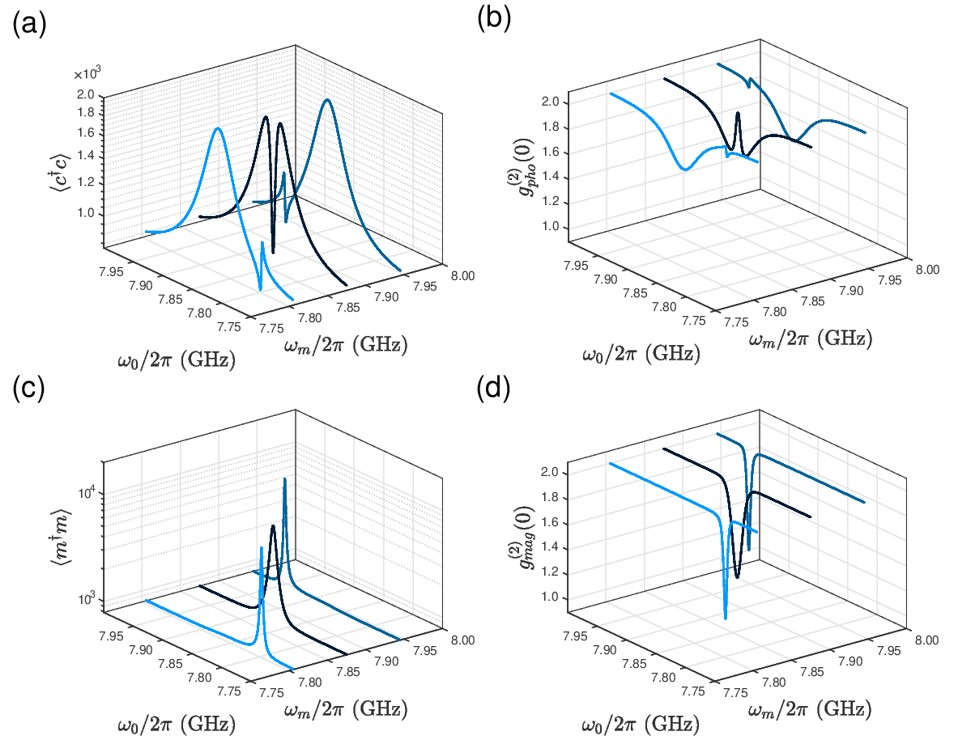
\includegraphics[width=2\basefigurewidth,clip]{./figure/4_6}
	\caption{MIT参数时不同磁场下光子和磁振子的稳态谱线} 
	\label{MITOmVary}
\end{figure}
如图\ref{MITOmVary}所示,我们在磁振子频率$\omega_m/2\pi$分别取7.805GHz,7.875GHz,7.945GHz时计算系统中平均粒子数与二阶关联函数的稳态谱线,其他参数为:$\omega_c/2\pi=7.875$ GHz, $\kappa_c/2\pi=30$ MHz, $\kappa_m/2\pi=1.06$ MHz, $g/2\pi=10.8$ MHz, $\Omega/2\pi=1$ GHz 以及 $T=300$ K。可以看到,在光子和磁振子的频率共振时,平均光子数的稳态谱线就是对称的MIT线型。而当二者远离共振的时候,本来出现在共振频率处的凹陷,我们称之为MIT窗口就会随着磁振子的频率而移动,并在磁振子频率附近出现了一个反对称的线型,也就是法诺线型。法诺共振广泛存在于有着背景和共振散射干涉的系统之中,通常使用法诺因子来表征这一非对称线型。我们这里的法诺因子可以由公式\eqref{first_order}导出,在远离共振的条件下$(\omega_c-\omega_0)\approx(\omega_c-\omega_m)$可以将光子的相干部分表示为
\begin{equation}
|\overline{\alpha_{0}}|^{2} =\frac{\Omega^{2}}{\kappa_{c}^{2}+(\omega_{c}-\omega_{m})^{2}}\frac{(q\Gamma+\omega_{0}-\omega_{1})^{2}}{\Gamma^{2}+(\omega_{0}-\omega_{1})^{2}}
\label{FanoEq}
\end{equation}
其中
\begin{gather}
\Gamma=\frac{g^{2}\kappa_{c}}{\kappa_{c}^{2}+(\omega_{c}-\omega_{m})^{2}} \\
\omega_{1}=\omega_{m}-\frac{g^{2}(\omega_{c}-\omega_{m})}{\kappa_{c}^{2}+(\omega_{c}-\omega_{m})^{2}}
\end{gather}
公式\eqref{FanoEq}中的参数 $q=(\omega_{m}-\omega_{c})/\kappa_c$ 即为法诺因子。从图\ref{MITOmVary}(a)中可以看出当法诺因子的正负性改变时,法诺线型的对称性也会跟着改变。在光子数的稳态谱表现出对称和非对称线型的时候,磁振子数的稳态谱一直保持着单峰并会随着偏置磁场改变位置,表现为铁磁共振的特征。

\subsection{腔磁振子系统中的Purcell效应}
\begin{figure}[htbp]
	\centering
	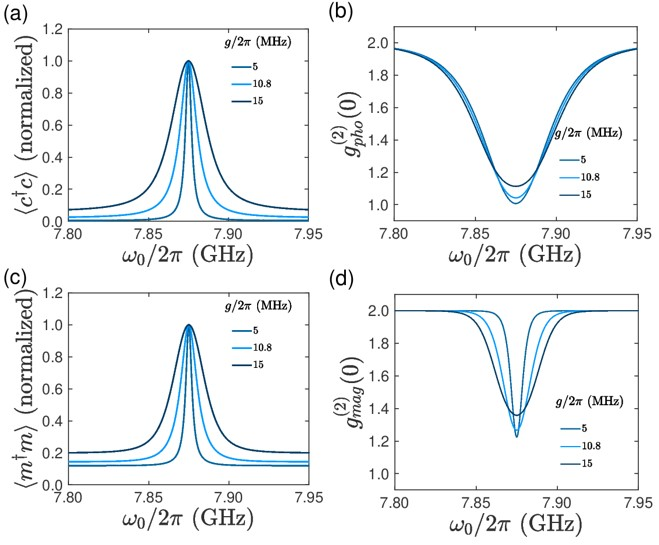
\includegraphics[width=1.9\basefigurewidth,clip]{./figure/4_8}
	\caption{腔磁振子系统中的Purcell效应} 
	\label{PurcellgVary}
\end{figure}
在Tang的实验中,当腔磁振子系统中耦合参数满足$\kappa_m>g>\kappa_c$时,测量结果还会表现出Purcell效应的特征。Purcell效应告诉我们光场与其他体系的耦合会引起光谱线宽的增强,这一增强的效果以一线型因子,即Purcell因子来表征。从图\ref{PurcellgVary}中我们可以直观看到Purcell增强的效应,当耦合率$g/2\pi$按照$5$MHz,$10.8$MHz,$15$MHz顺序增大时光子和磁振子的稳态谱线宽都会随之增宽,其中参数设置为:$\omega_c/2\pi=\omega_m/2\pi=7.875$ GHz, $\kappa_c/2\pi=1.35$ MHz, $\kappa_m/2\pi=30$ MHz, $\Omega/2\pi=1$ GHz 以及 $T=300$ K。而此时的Purcell因子同样可以由公式\eqref{first_order}导出,我们将一阶变量$\overline{\alpha_{0}}$整理为洛伦兹形式
\begin{equation}
\overline{\alpha_{0}}=\frac{\Omega}{i(\omega_{c}-\omega_{0})+\kappa_{c}\left(1+\frac{g^{2}}{\kappa_{c}\kappa_{m}}\frac{1}{1+\frac{i(\omega_{m}-\omega_{0})}{\kappa_{m}}}\right)}
\label{PurcellLine}
\end{equation}
当 $\kappa_m\gg(\omega_{m}-\omega_{0})$ 时,公式\eqref{PurcellLine}就变为了表示洛伦兹线型的公式,其洛伦兹线宽为 $\kappa_c(1+\frac{g^{2}}{\kappa_{c}\kappa_{m}})$。因此,我们说此时的光子数稳态谱在峰值附近处有着洛伦兹型的线型,而与磁振子的耦合导致了其洛伦兹线宽以Purcell因子$(1+\frac{g^{2}}{\kappa_{c}\kappa_{m}})$为倍数增强。

另一方面,我们还可以如图\ref{MITkcVary}一样,在改变磁振子的耗散率$\kappa_m$时观察稳态谱线是如何从强耦合转变为Purcell效应线型的。
\begin{figure}[htbp]
	\centering
	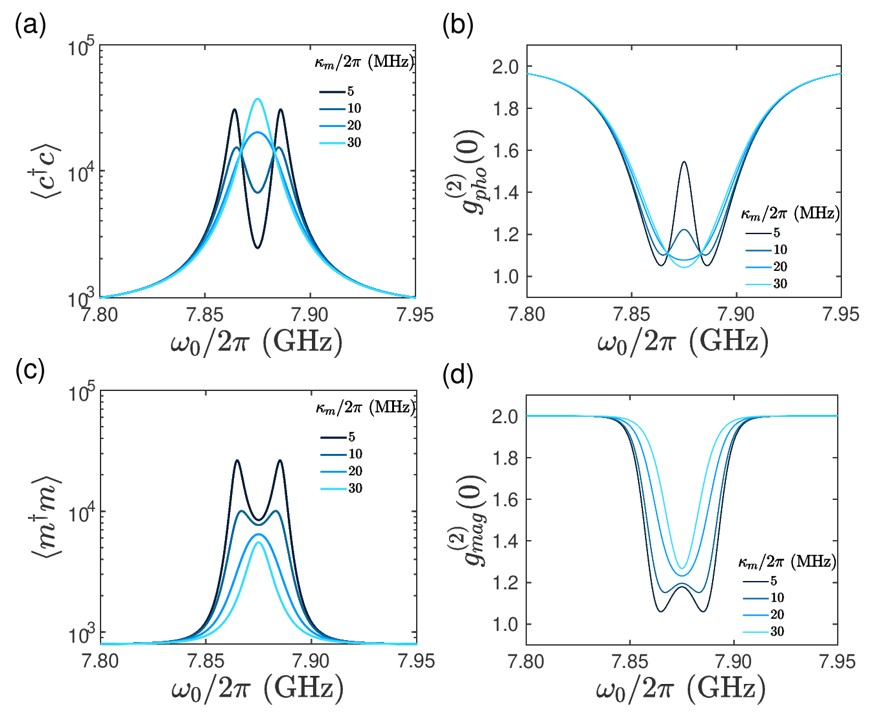
\includegraphics[width=1.9\basefigurewidth,clip]{./figure/4_7}
	\caption{磁振子耗散率增大时光子和磁振子的稳态谱线} 
	\label{PurcellKmVary}
\end{figure}
选取参数:$\omega_c/2\pi=\omega_m/2\pi=7.875$ GHz, $\kappa_c/2\pi=1.35$ MHz, $g/2\pi=10.8$ MHz, $\Omega/2\pi=1$ GHz 以及 $T=300$ K,计算$\kappa_m/2\pi$分别为$5$MHz,$10$MHz,$20$MHz,$30$MHz时的光子和磁振子稳态谱线如图\ref{PurcellKmVary}所示。在$\kappa_m/2\pi$增大的过程中,光子和磁振子稳态谱线都逐渐从双峰过渡为单峰。在$\kappa_m>g$之后,系统中的耦合地位逐渐降低,光子表现出解耦合的单峰线型,从Purcell因子可以看出,在$\kappa_m$增大到一定程度之后增强倍率会趋近于1。而磁振子耗散的增大使得稳态的相干磁振子数越来越少,$g_{mag}^{(2)}(0)$越来越趋近于2,磁振子也逐渐转变为热态。
